\chapter{Religion}
\section{Übersicht}
\begin{itemize}
	\item Der Glaube an 5 gute und 2 böse Götter.
	\item Das Symbol der Religion ergibt sich wie in Abschnitt \ref{sec:goettersymbol} erklärt aus dem Zusammenspiel der 7 Götter und ist in Bild \ref{fig:goettersymbol} dargestellt.
\end{itemize}

\begin{figure}
	\centering
	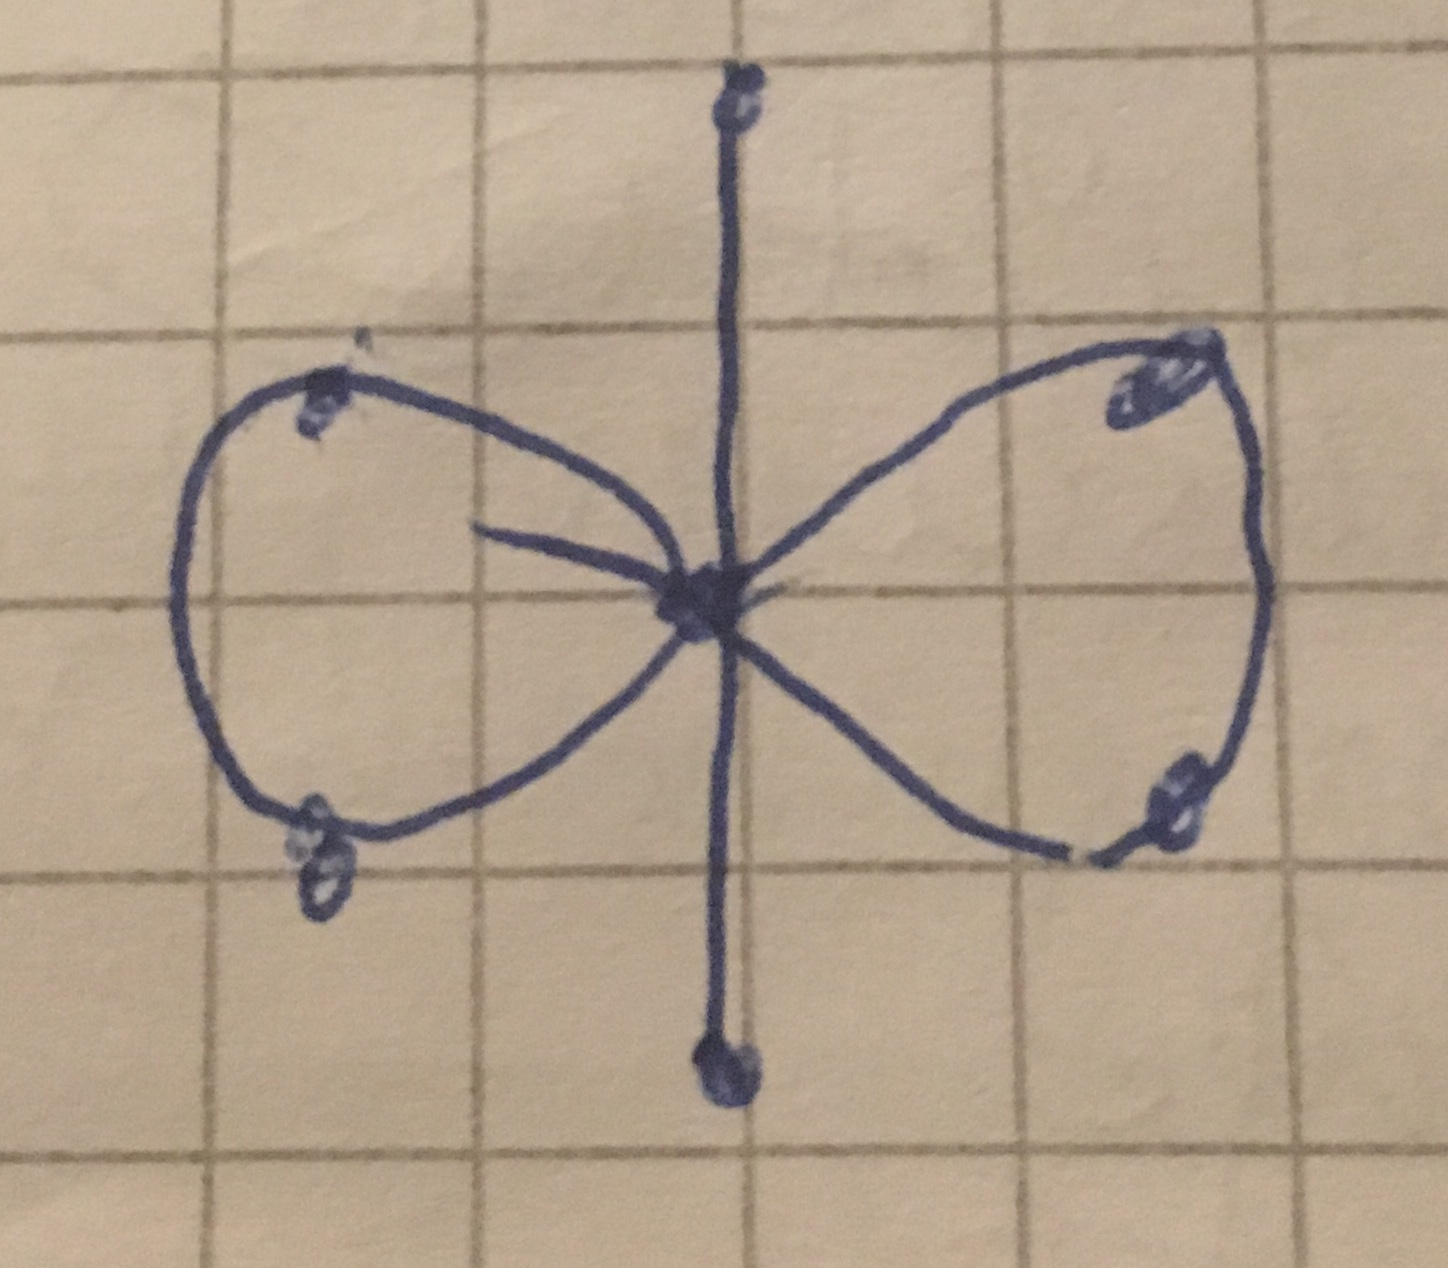
\includegraphics[width=0.3\textheight]{Abbildungen/Gesellschaft/Goettersymbol}
	\caption[Göttersymbol]{Das Symbol für die Götter}
	\label{fig:goettersymbol}
\end{figure}

\section{Geschichte}
Die hier erzählte Geschichte ist die vom Klerus verbreitete Sage über die Entstehung der Götter des Streits und der Heimtücke. \\\\
Es ist unklar, wie die Götter entstanden sind. Es geschah irgendwie irgendwann. Auf der noch recht unbewohnbaren Erde formten sie lebensfreundliches Gebiet mit ihrer jeweiligen Magie. Sie erschufen das Leben und ließen ihm seinen eigenen Lauf.\\
Nachdem sie jedoch viel Zeit damit verbracht hatten, sich an ihrem Paradies zu ergötzen, wollten sie auch Wesen nach ihrem Abbild schaffen und so lenkten sie das Leben und die Natur und brachten dadurch die Menschen hervor. Die Menschen, intelligent genug um Kultur aufzubringen, verfielen jedoch in viele Kriege. Mitgerissen aufgrund ihrer Ähnlichkeit und weil sie die Menschen so interessant fanden, integrierten sich die Götter in diese Streitigkeiten. Dabei nahmen sie die Positionen ihrer Menschengruppen an und halfen ihnen und wurden so langsam auch in einen Streit untereinander gezogen, wobei sie ihre negativen Seiten ausspielten.\\
Dies äußerte sich in vielen kleinen Dingen \textbf{(hier Geschichtchen einfügen)}, bis die Götter schließlich merkten, dass es so nicht weiter gehen kann. Sie setzten sich zusammen und kamen zum Schluss, dass sie, um wahre Leiter und Lenker des Lebens zu sein, ihre negativen Aspekte los werden müssten. Andernfalls würden ihre dunklen Seiten sie immer wieder übermannen können, was bereits große negative Folgen für alle Lebewesen hatte und auch wieder haben könnte.\\
Darum bereiteten die Götter ein Ritual vor, um perfekt zu werden und sich wortwörtlich von ihren schwachen Seiten rein zu waschen. Dazu begaben sie sich in einen See weitab der Zivilisation. Sie wuschen ihre schlechten Seiten von sich ab und versiegelten diese im See. \textbf{Allerdings gibt es ein kleines Leck, durch welches kontinuierlich ein wenig von der Magie und dem Schlechten austritt.}\\
Danach treten die Götter lange Zeit nicht in Erscheinung. In der Nähe des Sees, den Bach hinunter, lebte ein Paar. All sein Trinkwasser nahm es aus dem Bach und all ihre Ernte wurde mit dem Wasser bewässert. So nahmen sie über Zeit immer mehr von dem Bösen in sich auf. So wie ihre Macht und Magie wuchs, tat es auch das Böse in ihnen und verzehrte ihre guten Geister. Sie begannen aktiv das Böse aus der Umwelt und schließlich dem See zu absorbieren und wurden immer mächtiger und verdorbener. Sie führten Verwüstung und Zwist herbei und die Götter wurden auf sie aufmerksam. Ihre Versuche, sie zu bekämpfen und unter Kontrolle zu bekommen, scheiterten unter großen Verlusten in der Umwelt. Schließlich sahen die Götter ein, dass sie die beiden nicht besiegen konnten und unter all ihrer gebündelten Macht, um alle Lebewesen zu schütze, ersannen sie einen radikalen Plan.\\
Da die Götter zu verantworten hatten, dass diese Monster auf die Welt kamen, sahen sie es als ihre Pflicht, die Welt auch wieder von ihnen zu befreien. Aufgrund der zuvor genannten Umstände war die Maßnahme jedoch von drastischer Natur: sie hoben den Ort, auf dem sie die beiden bekämpften, aus der Erde heraus in den Himmel. Dort werden sie nun für alle Zeit gegen die beiden kämpfen und sie in Schach halten, damit das Leben auf der Erde geschützt ist.\\
Doch die beiden Bösen versuchen ihre Macht zu vergrößern, indem sie ihre Aktuelle auch dazu nutzen, den Lebewesen auf der Erde Böses einzuflüstern und sie zu manipulieren. \textbf{Die Erdenwesen sollen ihnen dienen.}\\
Bevor die guten Götter die Erdmasse mitsamt den Bösen in den Himmel aufgehoben haben, \textbf{erschufen sie gemeinsam einen Führer für die Toten}, der die verstorbenen Seelen zu ihnen bringen soll. Im Laufe der Zeit, in der sie ihre Pflichten als Götter und Führer der Welt etwas außen vor ließen, haben sie es geschafft, die Bösen zurück zu treiben. Nun gibt es nur noch Kampf auf einem kleinen Teil des Himmels-Brockens.\\
Nachdem die Toten verbrannt wurden, steigen ihre Seelen in den Himmel auf. Wenn die Verstorbenen in ihrem Leben gut waren und sich nicht von den Einflüsterungen der bösen Götter haben verführen lassen, werden sie vom Seelenleiter hinüber geführt, auf dass sie mit ihrer Kraft die Götter unterstützen und in ihrem Paradies wohnen können. Die verdorbenen Seelen jedoch werden vom Seelenleiter in die Irre geführt, damit sie nicht den Bösen helfen können, und verlieren sich in der unendlichen Dunkelheit.

\section{Götter}
In dem Land, in dem wir uns befinden, gibt es mehrere Götter. Regional unterscheidet sich die Wahl der bevorzugten Götter.
Diese sind Fiktion und existieren nicht wirklich; es gibt also auch keine Wunder, die von ihnen gewirkt werden. Allerdings interpretieren Menschen ja gerne sehr viel und sehen deshalb ein paar Dinge als Wunder an, die z.B. von den Priestern gemacht werden. Weil diese Priester gute Magier sind, aber das alles natürlich als Geschenk der Götter sehen.\\

\subsection{Das Göttersymbol} \label{sec:goettersymbol}
Beim Wasser-/Reinigungsritual, dem Abtrennungsritual oder einem anderen war die Aufstellung der fünf Götter und ihr Energiefluss wie dargestellt in Abb. \ref{fig:goetteraufstellung}. Denn die stärksten und direktesten Verbindundungen/Folgen ihrer Aspekte sind so. Das ergibt eine liegende acht, also das Symbol für Unendlichkeit --> 8 als heilige Zahl; Götter und ihre Macht sind unendlich.\\
\\
Mit den zwei Bösen Göttern: diese versuchen, alles zu spalten und zu zerstören. Das wird deutlich durch die Linie, welche die 8 versucht zu zerschneiden. Zudem zeigt es aber auch, wie durch die bösen Götter und zum Schutz des Lebens, ein Stück von der Erde abgetrennt werden musste. Des Weiteren mahnt es, wie unsere Schlechten Seiten immer Versuchung und Untergang sind — aber sie sind auch ein Teil von uns und wir müssen lernen, damit umzugehen und ihnen zu widerstehen. Aus diesen Aspekten ergibt sich das endgültige Göttersymbol wie dargestellt in Abb. \ref{fig:goettersymbol}.\\

\begin{figure}
	\centering
	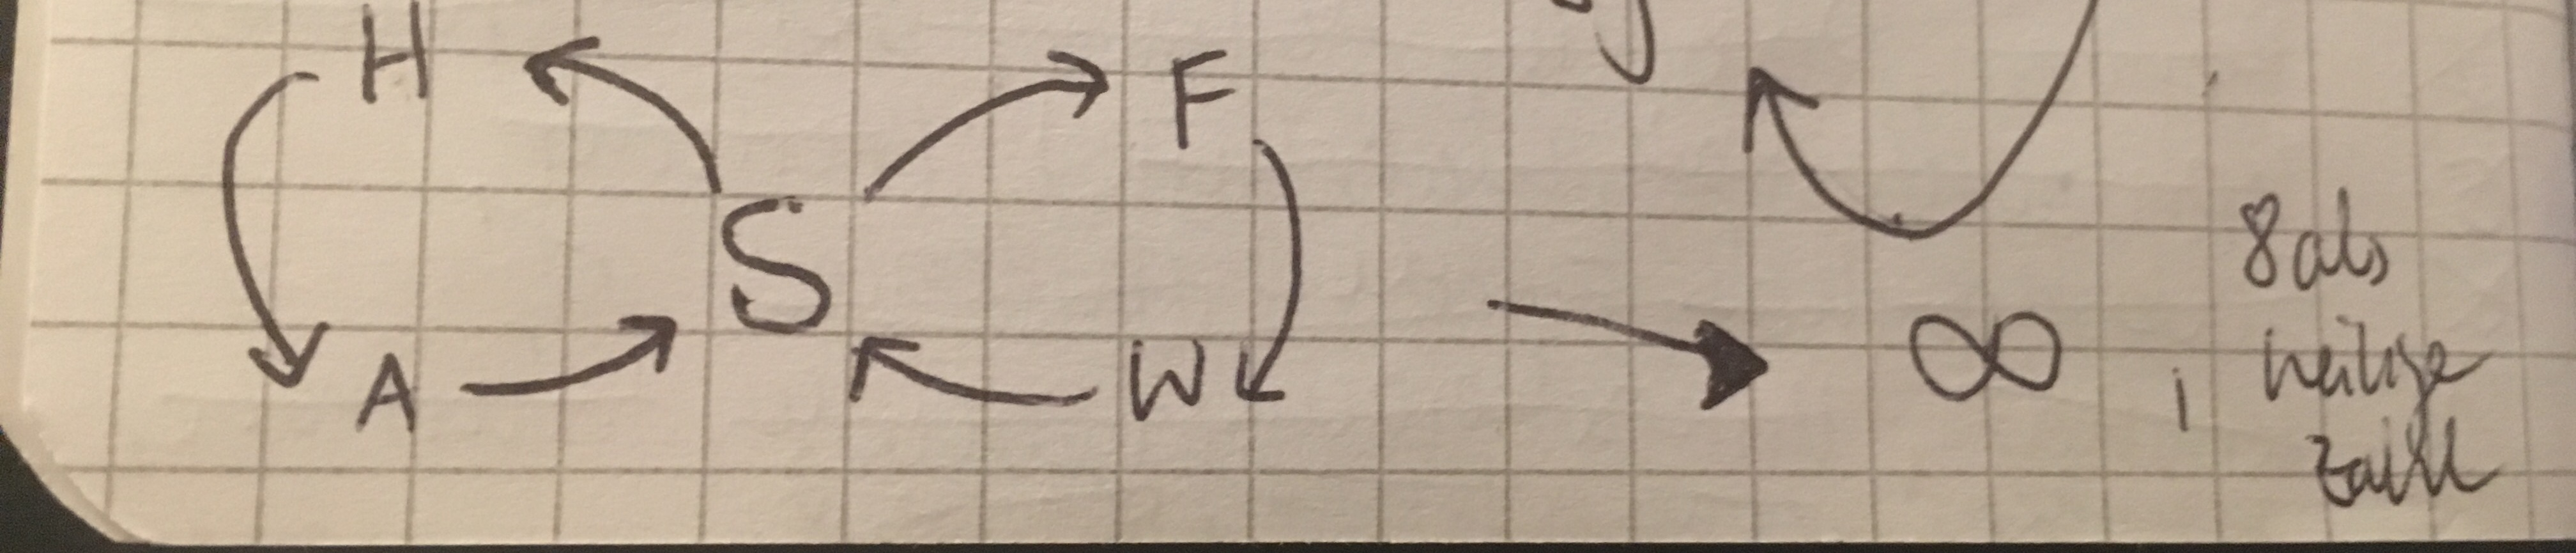
\includegraphics[width=0.7\linewidth]{Abbildungen/Gesellschaft/GoetteraufstellungbeiReinigungsritual}
	\caption{Aufstellung der Götter während des Reinigungsrituals}
	\label{fig:goetteraufstellung}
\end{figure}




\subsection{Gott des Schutzes}
männlich\\
Anführer der Götter\\
positive Aspekte: Mut, Macht, Kraft, Würde, Standhaftigkeit, Entscheidungsvermögen, Führungsqualitäten, Sicherheit, Intuition, Schutz\\
negative Aspekte: rücksichtslos, stolz, unterdrückend, hochnäsig, störrisch, grausam, überheblich, aggressiv, unanpassungsfähig, arrogant, egoistisch
\subsection{Göttin der Harmonie}
weiblich\\
positive Aspekte: Familie, Liebe, Selbstlosigkeit, Gnade, Mitgefühl, Vergebung, Demut, Reinheit, Frieden, Toleranz, Geborgenheit, Harmonie\\
negative Aspekte: aufgeben, rückgratslos, schwach, feige, scheu, abhängig, undiszipliniert
\subsection{Gott des Ausgleichs}
männlich\\
positive Aspekte: Höflichkeit, Aufstieg, Disziplin, Gleichgewicht, Ruhe, Gelassenheit, Geduld, Wachstum, Ausgeglichenheit, Strenge, Heilung, Ausgleich\\
negative Aspekte: Faul, neidisch, gefühllos, unberechenbar, unaufmerksam, charakterlos, jähzornig
\subsection{Gott der Freude}
männlich\\
positive Aspekte: Glück, Hingabe, Enthusiasmus, Fröhlichkeit, Freiheit, Menschlichkeit, Kunst, Kultur, Charme, Kreativität, Freude\\
negative Aspekte: wollüstig, völlernd, frech, eitel, misstrauisch, zynisch, nervös, voreilig, schadenfreudig, chaotisch, instabil, manisch
\subsection{Göttin der Weisheit}
weiblich\\
positive Aspekte: Erleuchtung, Wissen, Verständnis, Konzentration, Wahrheit, Klarheit, (Um-)wandlung, Zielstrebigkeit, Weisheit\\
negative Aspekte: eingebildet, versteift, zwingend, gierig, ängstlich, heimtückisch, habsüchtig, fanatisch, manipulativ, selbstüberschätzend, streitsüchtig
\subsection{Gott der Heimtücke}
männlich\\
positive Aspekte: \\
negative Aspekte: 
\subsection{Göttin des Streits}
weiblich\\
positive Aspekte: \\
negative Aspekte: 

\section{Klerus}
\textbf{Hier soll eine genauere Beschreibung des tatsächlichen Klerus erfolgen, also dem Teil der Struktur, der die Inhalte der Religion übermittelt. Zum Teil, der das Land verwaltet, siehe bitte \npref{ch:regierung}.} 

Da die Fähigkeit zur Nutzung der Magie natürlich auch von den Göttern kommt (nur wenige Arten können dies, ein paar Pflanzen, ein paar Tiere und darunter die menschlichen Arten (und unbekannterweise natürlich auch Mikroorganismen)), ist die Intensität, in der man Magie nutzen kann, natürlich auch ein Zeichen für die Gunst der Götter. Demnach müssen solche Leute stark in der Gunst stehen und daher auch ihr Leben den Göttern widmen - aka in den Orden gehen. Tatsächlich ist das aber auch ein Mittel des Ordens, diese mächtigen Leute zu kontrollieren, da sie die nach ihrer Art prägen und unter ihrer Anweisung haben

\subsection{Aufbau \& Struktur}

\subsection{Riten}
\paragraph{Ideen}
\begin{itemize}
	\item Predigt --> worshipping mit Gesang
\end{itemize}

\subsubsection{Tod}
Wenn jemand stirbt, so muss er verbrannt werden, damit seine Seele vom Körper frei wird und in den Himmel zu den Göttern aufsteigen kann und ihnen im Kampf gegen die bösen Götter beistehen kann. Das sollte optimal dann erfolgen, wenn die zweite Erde am Himmel steht, damit er schnell dort hingelangt. 
Gotteslästerer und böse Leute werden nicht verbrannt, sondern begraben oder ins Wasser geworfen (offenes Meer). So können sie den Bösen Göttern nicht beistehen.
Demnach ist es sehr schlimm, wenn jemand nach seinem Tod nicht angemessen aufbereitet und vor allem verbrannt wird!

\subsection{Gebäude}
